\documentclass[tikz]{standalone}
\usepackage{pgfplots}
\usepackage{mathpazo}
\usepgfplotslibrary{polar}
\usepgflibrary{shapes.geometric}
\usetikzlibrary{calc}
\usetikzlibrary{datavisualization}
\usetikzlibrary{datavisualization.formats.functions}
\pgfplotsset{compat=1.12} 
\pgfplotsset{my style/.append style={axis x line=middle, axis y line=middle, xlabel={$x$},ylabel={$y$},smooth}}
\begin{document}
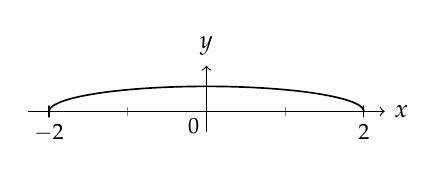
\begin{tikzpicture}[scale=1]
\datavisualization [school book axes, visualize as smooth line/.list={mynode},x axis ={label=$x$,ticks={step=2,minor steps between steps=1}},y axis ={label=$y$}]
%{major={at={0.05,0.10,0.15,0.20}}}}]%step=0.05,minor steps between steps=1}}]
data [format=function] {
var t : interval [0:pi];
func x = 2*cos(\value t r);
func y = 1/(pi)*sin(\value t r);
};
\end{tikzpicture}
\end{document}